\documentclass{article}[18pt]
\usepackage{../../../../format}
\lhead{Networks and Systems - Compiler Design}
\newtheorem{theorem}{Theorem}

\begin{document}
\begin{center}
\underline{\huge Finite Automata}
\end{center}
\section{Nondeterministic Finite Automata}
A nondeterministic finite automaton (NFA) consists of
\begin{itemize}
	\item A finite set S of states
	\item The input alphabet $\Sigma$ (the set of input symbols)
	\item A start state $s_0\in S$ (or initial state)
	\item A set F of final states (or accepting states)
\end{itemize}
Often we represent an NFA by a transition graph
\begin{itemize}
	\item Nodes are possible states
	\item Edges are directed and labelled
	\item The same symbol can label edges from a state to many different other states 
\end{itemize}
\subsection{Representation}
$$\Sigma = \{a,b\}$$
$$s_0=0$$
$$F=\{3\}$$
\begin{center}
	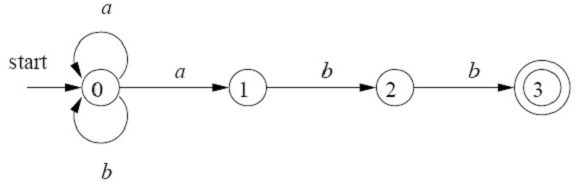
\includegraphics[scale=0.7]{NFA}
\end{center}
Alternative representation is a transition table
\begin{itemize}
	\item Rows $\rightarrow$ states
	\item Columns $\rightarrow$ symbols in $\Sigma \cup \{\epsilon\}$
	\item Entries $\rightarrow$ Transitions between states
\end{itemize}
\begin{center}
	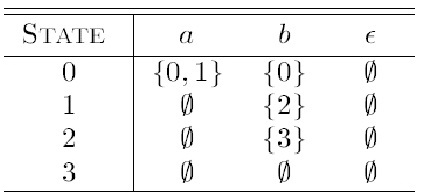
\includegraphics[scale=0.7]{NFA1}
\end{center}
Advantage of transition table: more visible transitions\\
Disadvantage of transition table: needs more space than the transition graph
\subsection{Acceptance of NFA}
An NFA accepts an input string x if there exists a path that:
\begin{itemize}
	\item Starts at the start state $s_0$
	\item Ends at one of the accepting states in F
	\item Concatenation of the symbols on its edges gives exactly x
\end{itemize}
A language accepted (or defined) by an NFA:
\begin{itemize}
	\item The set of strings that this NFA accepts
\end{itemize}
\section{Deterministic Finite Automata}
A deterministic finite automaton (DFA) is a special case of a NFA, where:
\begin{itemize}
	\item No edge is labelled by the empty string $\epsilon$
	\item For each state s and each input symbol a, there is exactly one edge out of s labelled with a
\end{itemize}
A direct algorithm to decide whether a given string x is accepted by a DFA:
\begin{itemize}
	\item Start at the start state $s_0$
	\item Iteratively follow the edges labelled by the characters of x
	\item Check whether you reach a final state when x ends:
	\begin{itemize}
		\item If yes, then the DFA accepts x
		\item Otherwise not
	\end{itemize}
\end{itemize}
\section{NFA vs DFA}
\begin{theorem}
NFAs accept exactly the regular languages (i.e. the regular expressions)
\end{theorem}

Therefore, simulation of an NFA can be used in the lexical analyser to recognise strings, identifiers etc\\
\\
However the simulation of NFAs is not straightforward
\begin{itemize}
	\item Many alternative outgoing edges from a state
	\item Transitions labelled with $\epsilon$ are possible
\end{itemize}
\begin{theorem}
	NFAs accept exactly the same languages as DFAs
\end{theorem}
i.e. for every NFA, we can construct an equivalent DFA
\section{From regular expressions to NFA}
\textbf{Our aim}: given a regular expression r, construct a NFA that accepts r\\
\\
Recursive construction\\
For any symbol $a\in \Sigma \cup \{\epsilon\}$ 
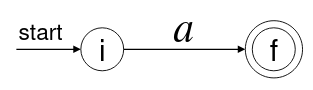
\includegraphics[scale=0.6]{recusrive}\\
\\
For any two regular expressions s and t with NFAs N(s) and N(t).
\newpage
If $r=s|t$
\begin{center}
	\includegraphics[scale=0.7]{"Two Regular Expressions"}
\end{center}
if $r=st$ =, then:
\begin{center}
	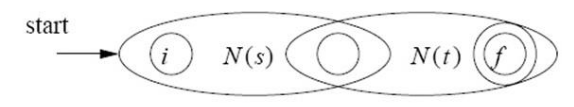
\includegraphics[scale=0.7]{r=st}
\end{center}
If $r=s^*$, then
\begin{center}
	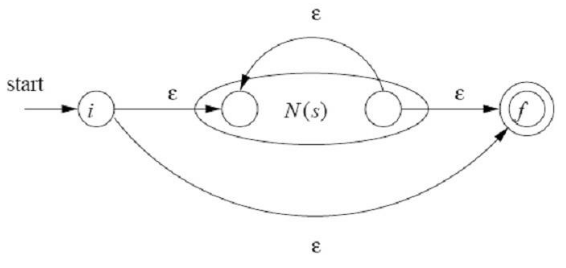
\includegraphics[scale=0.7]{r=s*}
\end{center}
\section{From NFA to DFA}
\textbf{Our aim}: Given an NFA, construct a DFA that accepts the same regular language. A DFA can be used directly as an automatic string/identifier recogniser.\\
\\
The main idea is that each state of the constructed DFA corresponds to a rest of states in the NFA\\
\\
Recursive construction of the DFA, after reading (any) input $a_1a_2\ldots a_k$ the DFA is in the state that corresponds to the set of states that the NFA reaches when reading the same input.
\section{Extensions of DFA}
A context free language can be recognised by a push-down automaton (PDA). This is exactly the same as an NFA, with the addition of a stack
\section{Push-Down Automata}
A push-down automaton(PDA) is a tuple $(Q,\Sigma, \Gamma, \delta, p, Z, F)$, where:
\begin{itemize}
	\item Q is a finite set of states
	\item $\Sigma$ is the input alphabet
	\item $\Gamma$ is the push-down alphabet
	\item $\delta$ is a set of transitions
	\item $p$ is the initial state
	\item $Z$ is a push-down symbol, initially in the stack
	\item $F$ is the same set of finial states
\end{itemize}
In general a PDA is non-deterministic\\
\\
A move in a PDA consists of:
\begin{itemize}
	\item Reading a symbol of $\Sigma \cup \{\epsilon\}$
	\item Changing state
	\item Replacing the top symbol of the stack by a (possibly empty) string
\end{itemize}
Writing a symbol on the stack "pushes" all the other\\
A PDA accepts an input string x if it reaches:
\begin{itemize}
	\item Either a final state in F
	\item Or an empty stack ($\epsilon$)
\end{itemize}
After reading the input x
\begin{theorem}
	PDAs accept exactly the context free languages
\end{theorem}

\begin{theorem}
	Deterministic PDAs accept strictly fewer languages that nondeterministic ones
\end{theorem}






\end{document}